% !TEX root = ../main.tex
\section{Findings for the Entire Population}
  
  This section will go through the results from the survey based on the entire population. 
  \todo[inline, color=blue!60]{The data used in this section are preprocessed. The procedures can be found in section.}

	\subsection{Pattern Creation Time}
    Figure \ref{fig:avgpatterncreationtimepopulation} gives the pattern creation time in seconds for the three pattern types. By looking at the average creation time for patterns, patterns created for bank accounts have the highest creation time of 9.42 seconds while patterns created for smartphones have an average creation time of 8.24 seconds. 

    Figure \ref{fig:patterncreationtimeexperience} shows the average pattern creation time in seconds for respondents experienced with the Android Unlock Pattern. The graph reveals that both patterns created for shopping account and banking account are not affected by the participants experience with the Android Unlock pattern.

    Patterns created for smartphones have a lower response time for patterns created by respondents experienced with the Android Lock Pattern. Patterns created for smartphones by experienced respondents had an have an average creation time of 7.20 seconds while the patterns created for smartphones by unexperiences respondents had an average creation time of 8.40 seconds. The difference in average creation time results in a difference of 1.2 seconds. 

		\begin{figure}[H]
      \subfigure[Average pattern creation time (seconds)]{
        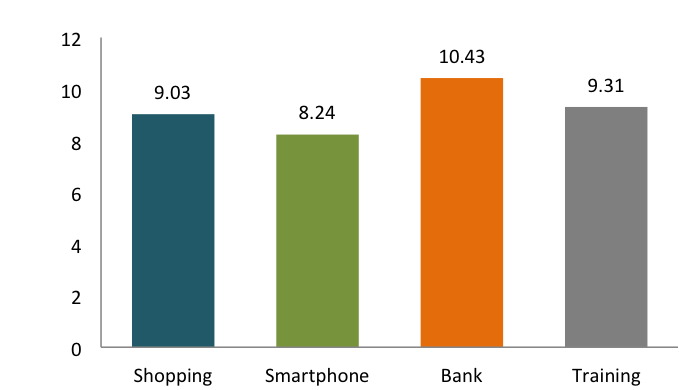
\includegraphics[scale=0.48]{pics/analysis/avgCreationTime.png}
        \label{fig:avgpatterncreationtimepopulation}
      }
      \subfigure[Creation time and experience with ALP]{
        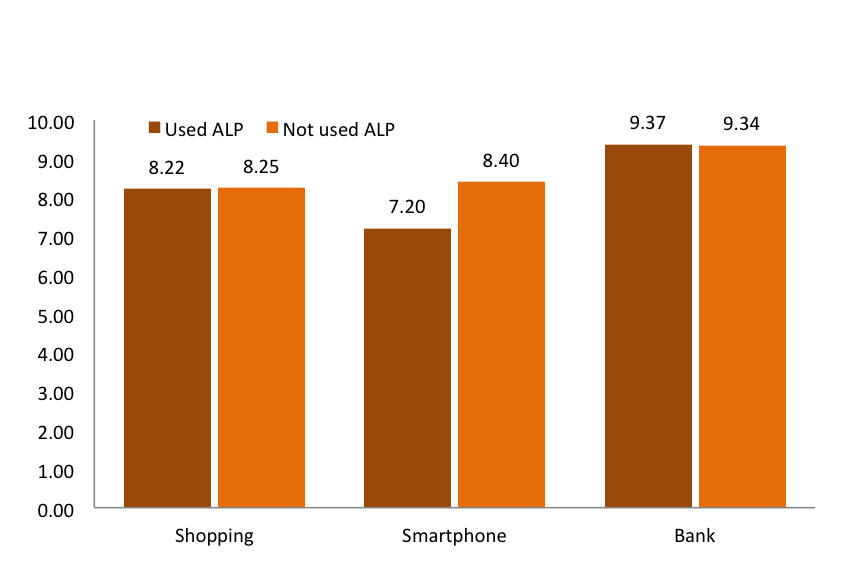
\includegraphics[width=0.48\textwidth]{pics/analysis/usedALPpatterncreationtime3.png}
        \label{fig:patterncreationtimeexperience}
      }
      \caption{Pattern creation time for the entire population}
      \label{fig:patterncreationtimepopulation}
    \end{figure}

  \clearpage
	\subsection{Pattern Length}

    Figure \ref{fig:avgpatternlengthpopulation} summarizes the average nodes selected to form a pattern for the each distinch pattern type. The average length is 5.54, 5.40, and 5.92 for patterns created for shopping accounts, smartphones, and bank accounts, respectively. The patterns created for bank accounts have a higher average length than patterns created for shopping and smartphone. The numbers from the graph also show that patterns created from smartphone has the smallest average pattern length. The difference in average pattern length for patterns created for smartphones and banking accounts are on average 0.52 nodes. Patterns created for shopping accounts are slightly longer than patterns created for smartphones but constitute not a significant difference between the two types.

    \begin{figure}[H]
      \centering
      \subfigure[Average Pattern Length (nodes)]{
        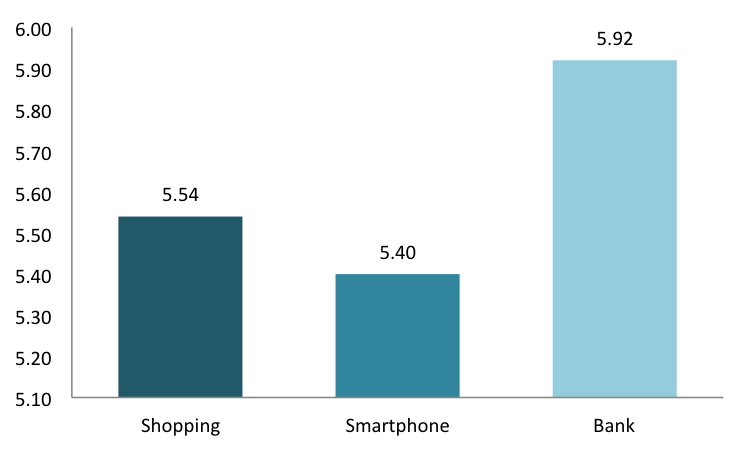
\includegraphics[scale=0.48]{pics/analysis/avgPatternLength.png}
        \label{fig:avgpatternlengthpopulation}
      }
      \subfigure[Pattern length distribution]{
        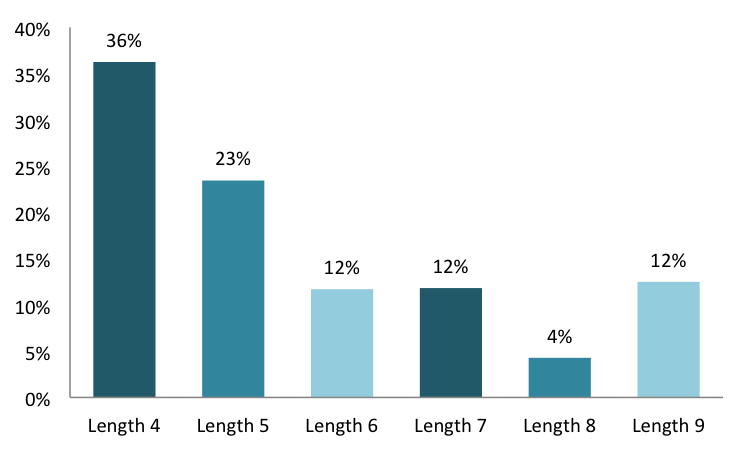
\includegraphics[width=0.48\textwidth]{pics/analysis/patternLength.png}
        \label{fig:patterndistpopulation}
      }
      \subfigure[Pattern length and type distribution]{
        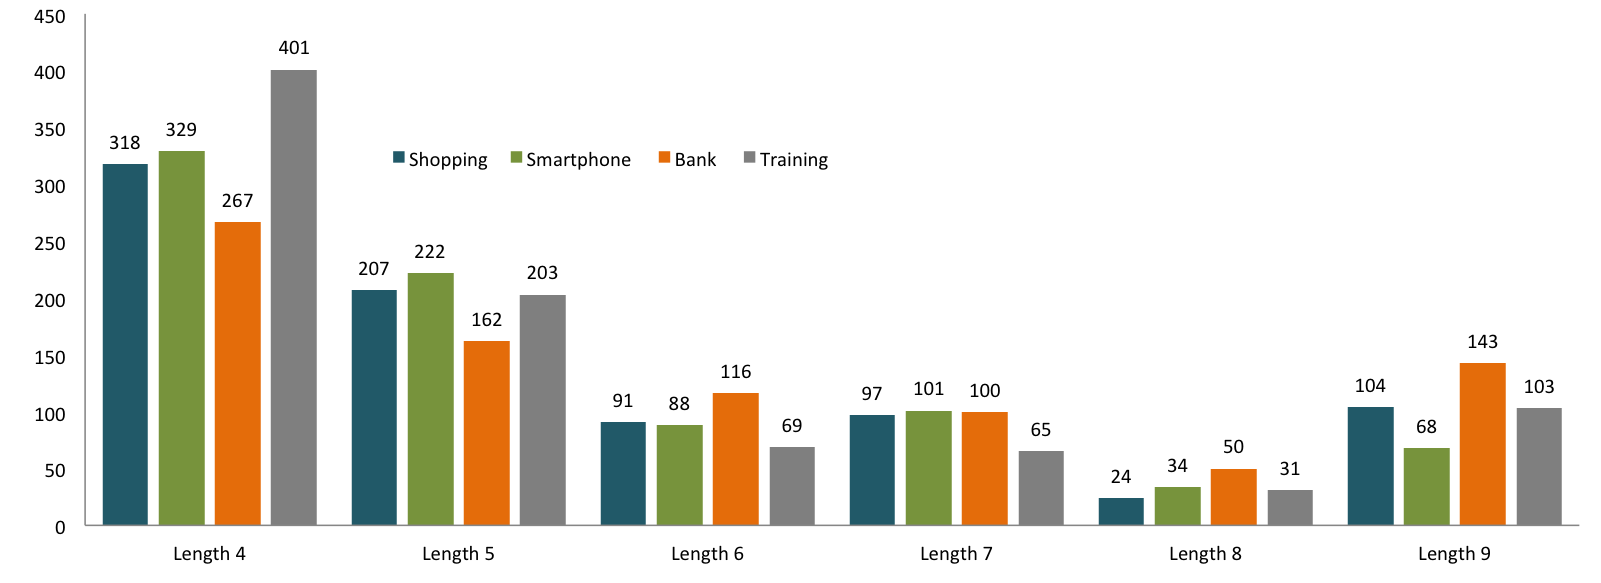
\includegraphics[width=\textwidth]{pics/analysis/patterntypePatternLength.png}
      \label{fig:patternTypePatternLength}
      }
      \caption{Pattern Length for the entire population}
      \label{fig:patternlengthpopulation}
    \end{figure}

    The graph in Figure \ref{fig:patterndistpopulation} is a pattern length distribution indicating what pattern length that are more often selected by the population. Figure \ref{fig:patternTypePatternLength} is a more detailed version of Figure \ref{fig:patterndistpopulation}, showing the pattern distribution for all pattern types. Both graphs give an indication the respondents selecting patterns having a length longer than 5 nodes less often. Both graphs in Figure \ref{fig:avgpatternlengthpopulation} and \ref{fig:patterndistpopulation} contains a low frequency of pattern with length 8, where patterns of length 7 and 9 both have a higher frequency than patterns of length 8.

    \clearpage
    The pattern created for shopping account and smartphones in Figure \ref{fig:patternlengthpopulation} have the majority of the patterns distributed over the shortest pattern lengths, e.g. patterns of length 4 and 5. Patterns created for banking accounts had the highest average pattern length, but the majority of the patterns created for bank accounts have still a length of 4 or 5.

	\subsection{Pattern Complexity}
  Table \ref{tab:patternstrength} is a summary of all the parameters used in calculating the strength of the patterns created by the entire population. The pattern length is not being further described as it was covered in the previous Subsection. The pattern length are named {\it Size} when talking about the length for calculating the visual complexity. 

  The physical length are increased when patterns utilize lines between the nodes that not are horizontal or vertical. A longer length are often correlated with the number of intersections and overlaps. Patterns created for bank accounts have the highest strength and highest occurrences of intersections and overlaps, 0.433 and 0.023 respectively. Patterns created for banking account also have a high pattern creation time and a high average pattern length. The average strength of patterns created for banking account are 15.514, also being the highest average strength score compared to the average score obtained by the two other types. 

  \begin{table}[H]
    \centering
      \begin{tabular}{l || l | l | l || l}
        \hline
        {\bf Parameters} & {\bf Shopping} & {\bf Smartphone} & {\bf Bank} & {\bf All} \\ \hline
        \#Patterns & 841 & 842 & 838                  & 2521 \\
        Avg. Size & 5.541 & 5.398 & 5.920             & 5.619 \\ 
        Avg. Length & 5.050 & 4.920 & 5.666           & 5.212 \\
        \#Intersections & 177 & 149 & 363             & 689 \\
        Avg. Intersections & 0.210 & 0.1769 & 0.433   & 0.273 \\
        \#Overlaps & 15 & 12 & 19                     & 46 \\
        Avg. Overlaps & 0.0178 & 0.014 & 0.023        & 0.018 \\ \hline
        Avg. Strength & 13.440 & 12.837 & 15.514      & 13.928 \\ 
        Min strength & 6.340 & 6.340 & 6.340          & 6.340 \\
        Max strength & 44.441 & 43.187 & 44.441       & 44.441 \\ \hline
    \end{tabular}
    \caption{Pattern strength for all patterns types in the entire population}
    \label{tab:patternstrength}
  \end{table}

  The smartphone is the pattern type with the weakest average strength. The characteristics of patterns created for smartphones is that they have a short pattern length in terms of number of nodes as well as a short physical length. The average occurrences of intersections and overlaps remain the lowest compared to patterns created for bank. The average number of occurrences of intersections and overlaps are 0.1769 and 0.014 respectively. The patterns created for smartphones gets an average strength score of 12.339, being the lowest score compared to the average score obtained by the two other types. Patterns created for shopping account are similar to patterns created for smartphones. All the parameters for patterns created for shopping accounts have slightly higher parameter values than for smartphone, hence a slightly higher average strength of 13.440.

  When looking at the maximum pattern strength of all patterns collected, none of the patterns obtained a maximum score of 46.8. In other words, none of the roughly 800 respondents managed to create a pattern obtaining a higher complexity score than 44.44. The set of patterns created for smartphones did include a pattern having obtained a  complexity score higher than 43.187, being a lower score than for the two other types

  \subsection{Association Elements} \label{sec:associationelements}
  An association element is something a person know or recognize, and can used as an element to ease the process of remembering a password. This is a known technique used by users when creating alphanumeric passwords and PIN codes. Alphanumeric passwords are often known being created containing personal information like names and dates for support the creator in remembering the password. The same strategy are being observed for PIN codes where the use of codes forming a date often occurs. 

  The dataset collected in this research are being scanned for patterns corresponding to association elements. By going through the alphabet, it was found 12 types of patterns corresponding to the visual representation of letters from the alphabet. Out of the 12 letters, 9 patterns had a significant number of appearances. Figure \ref{fig:associationpatterns} shows the 8 most common patterns having the same visual representation as letters from the alphabet. Beside the letters C, L, M, N, O, S, U and Z, letters like G, J and W also appeared in the data set.

  By iterating through the sequences corresponded to letter, 385 out of 3393 patterns in the dataset matched a letter. The number of patterns matching a letter from the alphabet constitutes 11.4\% of the collected patterns.

    \clearpage

      \begin{figure}[H]
        \centering
        \vspace{1.5cm}

        \subfigure[The letter C]{
          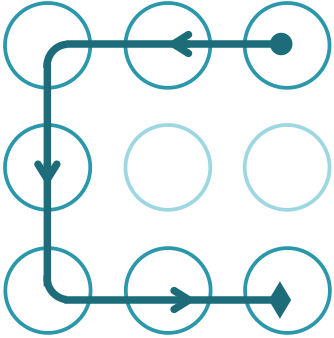
\includegraphics[width=0.27\textwidth]{pics/letters/bokstavenC.png}\hspace{0.6cm}
        }
        \subfigure[The letter L (big)]{
          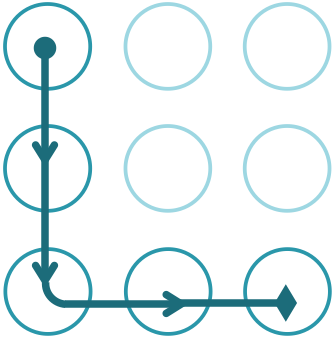
\includegraphics[width=0.27\textwidth]{pics/letters/bokstavenL.png}\hspace{0.6cm}
        }
        \subfigure[The letter L (small)]{
          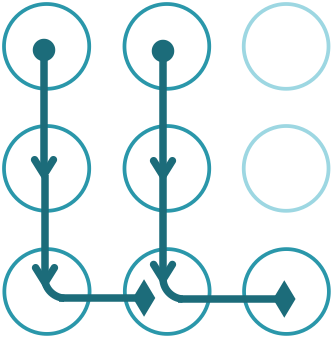
\includegraphics[width=0.27\textwidth]{pics/letters/bokstavenLitenL.png}
        }

        \vspace{0.5cm}

        \subfigure[The letter M]{
          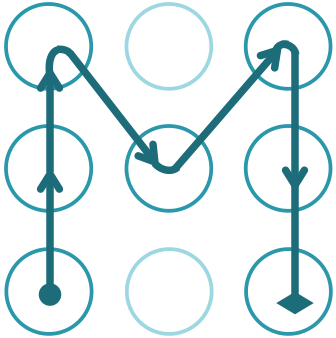
\includegraphics[width=0.27\textwidth]{pics/letters/bokstavenM.png}\hspace{0.6cm}
        }
        \subfigure[The letter N]{
          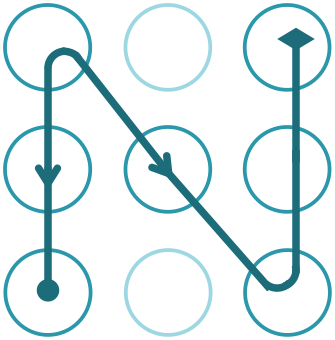
\includegraphics[width=0.27\textwidth]{pics/letters/bokstavenN.png}\hspace{0.6cm}
        }
        \subfigure[The letter O]{
          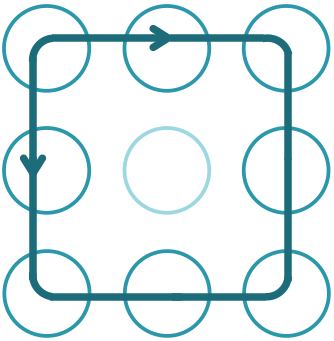
\includegraphics[width=0.27\textwidth]{pics/letters/bokstavenO.png}
        }

        \vspace{0.5cm}

        \subfigure[The letter S]{
          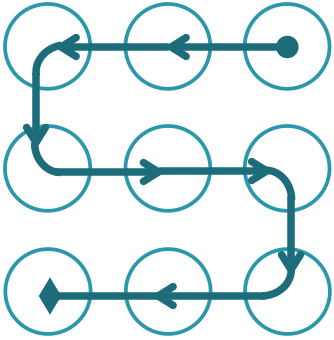
\includegraphics[width=0.27\textwidth]{pics/letters/bokstavenS.png}\hspace{0.6cm}
        }
        \subfigure[The letter U]{
          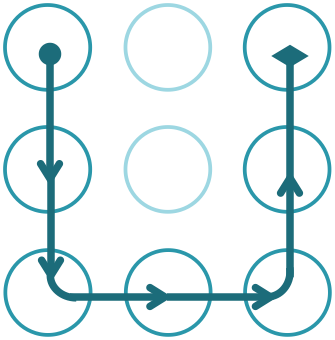
\includegraphics[width=0.27\textwidth]{pics/letters/bokstavenU.png}\hspace{0.6cm}
        }
        \subfigure[The letter Z]{
          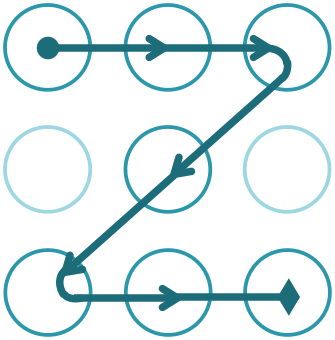
\includegraphics[width=0.27\textwidth]{pics/letters/bokstavenZ.png}
        }

        \vspace{0.5cm}
        \caption{Most frequent patterns forming letters from the alphabet}
        \label{fig:associationpatterns}
      \end{figure}

    \clearpage

  \subsection{Bias in the Selection of Start Node}
  
    The starting node of a pattern is a crucial information to have when analyzing patterns because of the properties of a legal pattern. A legal pattern can only visit the same node twice, making the starting point a help for excluding probable patterns.

    Table \ref{tab:startingNode1} is a summary of the likelihood of starting in a particular node for each of the four pattern types. The numbers notation used in the table, 1-3 and T, is a shortcut for the different pattern types shopping account (1), smartphone (2), banking account (3), and training (T). On average, 44\% of all patterns starts in node 1, e.g. the upper-left corner. 

    The training patterns are not included in other sections because there are no control over how many times a person have entered a tarining pattern. The training pattern are still valid when looking at the starting node because it reflects where respondents starts creating patterns. 

    %Table: Starting node dist
    \begin{table}[H]
      \centering
      \begin{tabular}{ c || c | c || c | c | c | c }
        \hline
        {\bf Start node} & All & 1,2,3 & 1 & 2 & 3 & T \\ \hline
        1 & 44\% & 42\% & 43\% & 41\% & 42\% & 51\% \\
        3 & 15\% & 15\% & 16\% & 14\% & 13\% & 14\% \\
        7 & 14\% & 14\% & 13\% & 15\% & 14\% & 13\% \\
        2 & 9\%  & 9\%  & 10\% & 9\%  & 8\%  & 7\%  \\
        4 & 6\%  & 7\%  & 6\%  & 7\%  & 7\%  & 6\%  \\
        5 & 4\%  & 4\%  & 4\%  & 4\%  & 4\%  & 3\%  \\
        9 & 4\%  & 4\%  & 3\%  & 3\%  & 5\%  & 3\%  \\
        8 & 2\%  & 3\%  & 2\%  & 3\%  & 3\%  & 2\%  \\
        6 & 2\%  & 2\%  & 2\%  & 2\%  & 3\%  & 2\%  \\ \hline
      \end{tabular}
      \caption{Selection of starting node for all pattern types}
      \label{tab:startingNode1}
    \end{table}

    Figure \ref{fig:startingNode3} is an illustration of the likeliehood of starting in the different nodes. Each node has a number, starting from node 1 in the upper left corner ending up with node number 9 as shown in Figure \ref{fig:startingNode2}. All nodes in Figure \ref{fig:startingNode3} are colored based on the likeliehood of being chosen as a starting point from high to low (green - blue - orange), whereas the green nodes are the most common starting points and orange nodes is the least common starting points.

    Summarizing the most common starting points, node 1, 2 and 7, they all together constitutes 73\% of the patterns. The different pattern types have all over 40\% of the patterns starting in the upper left corner. There are some nodes that are not a typical starting point. The nodes with the lowest frequency as starting point is the node 5,6,8 and 9 with only a total probability of 12\% of being selected as a starting node.

      %Figure: Staring node for all patterns
    \begin{figure}[H]
      \centering
      \subfigure[Node positions]{
        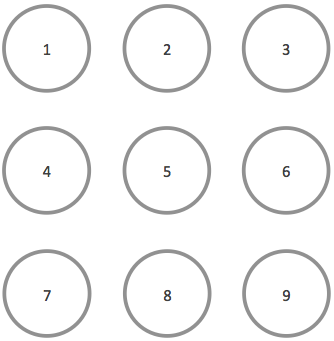
\includegraphics[scale=0.40]{pics/analysis/nodeposition.png}
        \label{fig:startingNode2}
      }
      \hspace{0.7cm}
      \subfigure[Staring node for all pattern types]{
        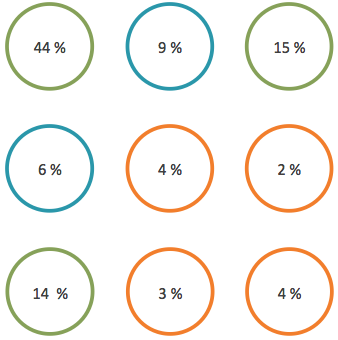
\includegraphics[scale=0.40]{pics/analysis/commonnode.png}
        \label{fig:startingNode3}
      }
      \caption{Node position and likely starting point for all pattern types}
      \label{fig:startingNode4}
    \end{figure}

  \subsection{3-gram Movement Patterns} \label{sec:3gram}
  
    \todo[inline, color=red!80]{Vise en liste med top mønstre og vise at x antall prosent velger passord som starter på samme måte.}
    %Figure: Most common 3-gram to less common 3-gram
    \begin{figure}[H]
      \subfigure{
        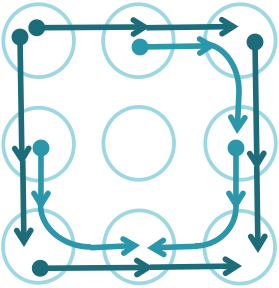
\includegraphics[width=0.31\textwidth]{pics/analysis/3gram1.png}
      }
      \subfigure{
        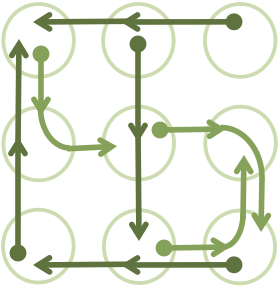
\includegraphics[width=0.31\textwidth]{pics/analysis/3gram2.png}
      }
      \subfigure{
        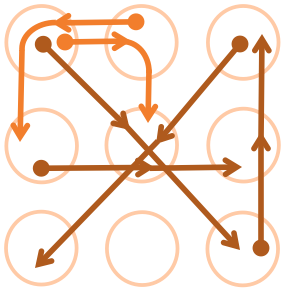
\includegraphics[width=0.31\textwidth]{pics/analysis/3gram3.png}
      }
      \caption{Most common 3-gram to less common 3-gram}
      \label{fig:3gram}
    \end{figure}
